% ---------------------------------------------------------------------
% CHAPTER 4 — \chapter{Method}
% 4.1 Cumulative Research Design
% The studies as a deliberate sequence, each taking up a limitation the previous left open
% Part I progression: NEGAR → GAER → ARL → StructSAR
% Part I → Part II transition: supervision changes, not the design space
% C2A study adds the graph-free control absent in recovery
% HetMap as capstone: independently varies file representation and graph structure under a matched encoder
% Why this is complementary progression, not replication

% 4.2 Unit of Analysis and Graph Representations

% The file as the unit clustered/classified; folders and members shape representation but are never prediction targets
% The four-rung ladder: file-only dependency → typed multi-relational file → folder–file → folder–file–member
% Ladder vs. relation modeling as independent but interacting choices

% 4.3 Signal Taxonomy

% Five signal categories: structural, organizational, lexical, contextual, interaction detail
% Why keeping them distinct matters for ORQ2 and ORQ3
% Studies differ in whether they fuse or isolate these signals

% 4.4 Learning Settings

% Unsupervised recovery: GAE / VGAE / DGI, clustering after training, module count searched
% Semi-supervised mapping: known target set, small labeled seed, iterative self-training
% Why metrics differ (ARI vs macro-F1) and why results are never pooled across settings

% 4.5 Controlled-Comparison Logic

% Controlled comparison as the search strategy, against joint optimization
% Three instances: graph-free MLP vs graph-based; dependency-only vs folder-augmented; HetMap's independent feature × graph variation
% A set of overlapping controlled comparisons, not a fully crossed factorial

% 4.6 Subjects, Ground Truth, and Evaluation Protocol

% Benchmark systems table (properties, homophily, degree, LoC, modules)
% Ground-truth provenance and status as expert judgment, not measurement
% Protocol: 100 runs, paired seeds, median, Wilcoxon signed-rank, Cliff's delta, Holm correction, per-system reporting

% 4.7 Threats Addressed by Design

% Metric dependence
% Ground-truth subjectivity
% Folder–reference correspondence confound
% Static dependency extraction error
% Stochasticity from initialization and training
% Cross-system heterogeneity as asset once results are not pooled
% ---------------------------------------------------------------------
\chapter{Research Method}
\label{ch:methodology}
\chaptertoc

This chapter presents the research methodology used to address the two problems this thesis studies, software architecture recovery and code-to-architecture mapping, through the graph-based representation-learning artifacts developed across its studies and the reasoning that connects them into one coherent design. It states the paradigm the studies share, how their progression from recovery to mapping was chosen rather than incidental, the unit and graph representations common to all of them, the taxonomy of input signals that recurs across studies, the two learning settings and what distinguishes the questions they can answer, the controlled-comparison logic used to decide when a design choice is justified, the systems and evaluation protocol the studies share, and the threats that this design addresses.

\section{Research Design}
\label{sec:research_design}

\subsection{Design Space}
\label{sec:design_space}

Architecture recovery and mapping are approached through a common graph representation, and the choices involved in constructing and initializing this representation define the design space studied in this thesis, summarized in Figure~\ref{fig:design_space}. This space varies along three independent axes: node types, edge types, and node features. On the node axis, a graph is homogeneous with a single node type, typically files, or heterogeneous with additional folder or member nodes. On the edge axis, a graph may merge all static dependencies into one relation or be multi-relational, preserving distinct dependency types such as \emph{call}, \emph{import}, and \emph{inheritance} as separate edges; a homogeneous or multi-relational graph built solely from these static dependencies is the SDG. In heterogeneous graphs, folder-to-file and file-to-member meta-relations connect nodes of different types, distinct from the static dependencies. On the feature axis, node representations may be initialized without external signals, using learnable identity embeddings, or from external signals such as folder path tokens, lexical identifiers, and contextual code embeddings, or omitted in favor of a graph-free baseline that isolates what message passing itself contributes.
\begin{figure}[!hbtp]
    \centering
    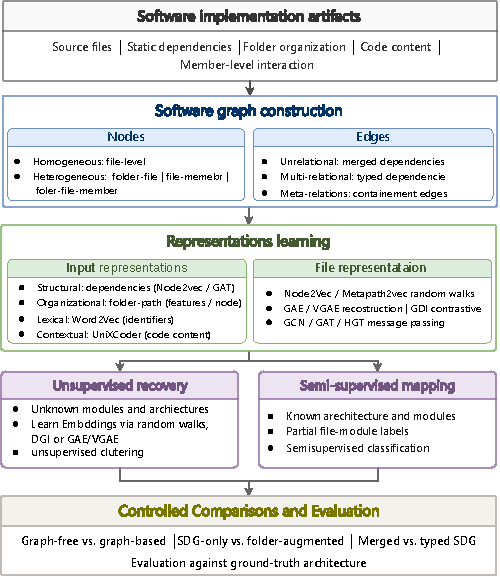
\includegraphics[width=1\textwidth]{figures/thesis_pipeline.pdf}
    \caption{Design space studied across the thesis. Software implementation artifacts are represented as graph configurations ranging from the homogeneous SDG to heterogeneous folder-file-member graphs. Structural, organizational, lexical, contextual, and interaction-level signals provide input representations, from which representation-learning methods derive file embeddings. These embeddings support unsupervised recovery and semi-supervised mapping and are evaluated against ground-truth reference decompositions. Across studies, controlled comparisons examine relation modeling, graph structure, input representations, and graph-based learning.}
    % \caption[Design space studied in the thesis.]{Design space studied across the thesis: graph configurations ranging from the SDG to heterogeneous folder-file-member graphs, initialized from structural, organizational, lexical, or contextual signals, and evaluated under unsupervised recovery and semi-supervised mapping through controlled comparisons of relation modeling, graph structure, input signal, and message passing itself.}
    % \label{fig:design_space}
\end{figure}

\subsection{Research Trajectory \label{sec:research_traj}}

The studies in this thesis form an incremental investigation of graph-based representation learning for architectural analysis, on the premise that architectural information is distributed across static dependencies, project organization, and source-code content. This framework integrates or isolates these sources: dependency relations define a file's structural context, while node and edge attributes encode organizational, lexical, contextual, or interaction-level information. Each study addresses limitations identified in the previous one, investigating how these sources should be represented and learned from, rather than assuming one graph construction, feature representation, or encoder is uniformly appropriate.

The prior graph-based representation learning approach to architecture recovery, NEGAR~\cite{negar}, learns file embeddings from SDG via node2vec-style random walks and clusters them into modules. It evaluates dependency types through separate pipelines and does not incorporate folder organization or lexical information. This leaves open whether typed dependencies can be modeled jointly and whether organizational and lexical signals provide complementary evidence for recovery. GAER~\cite{gaer} addresses this question by representing typed dependencies as relation-specific graph structures and combining folder paths and code identifiers as node features within a graph autoencoder framework. It further examines how encoder choice (GCN vs.\ GAT) and cluster granularity affect the results. However, because these signals are fused within the same configuration, the contribution of each source cannot be separated from the others.

A subsequent recovery study investigates a different self-supervised learning objective. It uses contrastive learning rather than graph reconstruction and augments file-level dependency edges with attributes that describe the member-level interactions that give rise to each dependency. This examines whether interaction type and frequency provide useful architectural information beyond the existence of a file-level dependency~\cite{arl_2026}. A further recovery study then examines dependency structure and project organization more directly. It compares dependency-only file graphs with folder-augmented heterogeneous graphs using both random-walk and graph-attention representation learners. The graph-attention variants are trained with a variational graph autoencoder, and the study additionally evaluates positional encoding~\cite{lpe} and diffusion-based structural augmentation~\cite{gdc} to extend the effective reach of shallow message-passing models~\cite{structsar}.

The remaining two studies turn to mapping source files to architectural modules, where the module set is known, and a subset of files is labeled. This study formulates mapping as semi-supervised node classification with iterative self-training over a multi-relational graph~\cite{mapping_ext}. It further introduces a graph-free multi-layer perceptron (MLP) baseline, trained under the same features and self-training procedure, to compare GNN-based prediction against feature-only prediction, a comparison absent from the recovery studies. The resulting difference indicates what the GNN encoder contributes beyond the file-level features, though it does not isolate message passing alone, since the models also differ in parameterization.

The final study extends this mapping design by introducing a dependency-guided contextual code representation and by expanding the graph to include folder and member nodes. It compares structural, lexical, and contextual representations both without message passing and as inputs to the same heterogeneous graph transformer, across graph variants that add or remove folder and member nodes. Thus, rather than directly validating all earlier results, it tests how these representations and graph structures contribute under one matched semi-supervised mapping setting.

% ============================================================
% Graph and Signal Representation
% Subsection 3 of 3 under Chapter 4, Section "Research Design"
%   (alongside: Design Space, Research Trajectory)
% ============================================================

\subsection{Graph and Signal Representation}
\label{sec:graph_signal_representation}

The design space defines the representational choices in the abstract. This subsection instantiates them concretely, showing which graph each study constructs and which signals it places on that graph's nodes and edges. Table~\ref{tab:graph_signal} summarizes both axes across the five studies; the prose that follows explains why each study sits where it does.

\subsubsection{Graph Construction}

The five studies construct their graphs at increasing levels of richness, each adding structure the previous studies could not represent. GAER and the architecture representation learning study model the system as a multi-relational, file-level SDG, keeping dependency types such as \emph{call}, \emph{import}, and \emph{inheritance} as separate, relation-specific edges; neither goes beyond file-level nodes. The controlled variational-GAE study isolates project organization from this file-level structure by comparing a single-relation SDG against the same graph augmented with folder nodes and folder--file containment relations, including a typed-dependency variant within that heterogeneous setting, to test whether organizational structure contributes beyond dependencies alone. The C2A mapping extension carries the multi-relational, file-level SDG into a supervised setting without extending its structure further. The heterogeneous graph study then adds member nodes that aggregate each file's methods and fields, connected by file--member containment alongside the existing folder--file containment and file--file dependency relations, reaching the finest granularity studied in this thesis.

\begin{table}[!t]
\caption{Graph construction and signal representation across the five studies. Edge attributes carry relation type only, except ARL-E, which adds interaction type and frequency, and StructSAR's diffusion variant, which attaches a personalized PageRank (PPR) edge weight.}
\label{tab:graph_signal}
\begin{threeparttable}
\begin{adjustbox}{max width=\textwidth}
\begin{tabular}{@{} l l l l @{}}
\toprule
\textbf{Study} & \textbf{Nodes} & \textbf{Dependencies} & \textbf{Node features} \\
\midrule
GAER & File & Multi-relational SDG & Path BoW $\Vert$ W2V ids \\
ARL / ARL-E & File & Multi-relational SDG & Path BoW $+$ id BoW \\
C2A mapping & File & Multi-relational SDG & Path BoW $\Vert$ W2V ids \\

\midrule
StructSAR& Folder, file & Single- or multi-relational & Learnable id ($+$LPE) \\
HetMap & Folder, file, member & Multi-relational & W2V / N2V / UniXcoder \\
\bottomrule
\end{tabular}
\end{adjustbox}
\begin{tablenotes}
\footnotesize
\item BoW = bag-of-words; W2V = Word2Vec; N2V = node2vec; LPE = Laplacian positional encoding.
\end{tablenotes}
\end{threeparttable}
\end{table}

\subsubsection{Input Signal Representation}

Node feature construction instantiates the feature axis of the design space at the study level. GAER and the C2A mapping extension initialize every file node from external signal, concatenating a binary file-path bag-of-words vector with an $\ell_2$-normalized average of Word2Vec embeddings over its code identifiers, so that organizational and lexical evidence enter the encoder together as one fixed input. The architecture representation learning study draws on the same two sources but encodes both as binary token vectors with $\ell_2$ normalization, using a bag-of-words encoding of identifiers in place of a separately trained lexical embedding. The controlled variational-GAE study uses no external node signal: each node type receives a learnable identity embedding trained with the model, and file nodes additionally carry a Laplacian positional encoding concatenated to that embedding, so the encoder is supplied with position in the dependency graph rather than folder or lexical content. Its random-walk baselines are a further case with no node feature vector at all, since node2vec and MetaPath2Vec learn embeddings directly from walk co-occurrence over the graph.

The heterogeneous graph study treats node initialization as the object of study rather than a fixed choice. It compares three external strategies for file and member nodes under otherwise matched conditions: lexical Word2Vec embeddings over identifiers, structural node2vec embeddings over the dependency graph, and contextual UniXcoder embeddings in both zero-shot and dependency-guided fine-tuned form. Folder nodes, when present, are always encoded from binary folder-path tokens irrespective of the strategy used for file and member nodes, keeping the organizational signal fixed while the file- and member-level representation varies.

Edge attributes form a narrower axis, extended beyond relation type in only two of the five studies; elsewhere edges carry their type alone and all relational evidence passes through multi-relational message passing. The architecture representation learning study augments its file-level edges with an attribute vector describing how each dependency arises, concatenating a binary, $\ell_2$-normalized encoding of the member-level interaction type that produced the dependency with a log-normalized count of how often that interaction occurs between the two files, testing whether the origin and frequency of a dependency add information beyond the presence of a typed edge. The controlled variational-GAE study attaches an edge attribute of a different nature in its diffusion variant, where graph diffusion convolution rewires the file graph through Personalized PageRank and gives each rewired edge a scalar weight that biases the attention logits toward diffusion-close neighbors. That weight is an artifact of the diffusion process rather than external content of the kind folder, lexical, and contextual features supply, so edge attribute initialization does not constitute a third input axis co-equal with node features. It is a targeted extension, used where a study's question concerns interaction semantics or the reach of shallow message passing.

\section{Learning Settings}
\label{sec:method-learning}

The two tasks are studied under different learning settings, and the settings answer related but not identical questions. Unsupervised recovery has no labels to train against, so a graph autoencoder or its variational form reconstructs observed graph structure from the learned representations, or a contrastive objective such as deep graph infomax trains the encoder by distinguishing the observed graph from a corrupted view, and the resulting file embeddings are clustered into modules after training. The number of modules is itself unknown and is searched over rather than fixed, so a recovery result is a partition whose granularity the method itself must choose. Semi-supervised mapping has a target module set that is known in advance and a small initial labeled set, so a classifier, built on a graph convolution, attention, or heterogeneous transformer encoder, predicts module membership directly, and the labeled set is expanded through iterative self-training as the model's own confident predictions are added back into the training data.

Clustering and classification are evaluated with different metrics for this reason, not only by convention. A clustering agreement measure such as the adjusted Rand index rewards a partition for resembling the reference regardless of how many clusters it contains, since the method was never told how many modules to produce, while a classification metric such as macro-F1 evaluates predictions against a fixed, known label set that the method receives as part of its supervision. This is why recovery and mapping results are never merged into one pooled statistic anywhere in this thesis: an improvement in ARI and an improvement in macro-F1 are answers to related but structurally different questions, and treating them as interchangeable would misstate what each setting can show.

\section{Controlled-Comparison Logic}
\label{sec:method-comparison}

The design space is not searched by optimizing over its dimensions jointly, which is the strategy this thesis positions itself against, since fixed weightings tuned once do not adapt across systems. It is searched by controlled comparison: within a study, one dimension is varied while the others are held fixed, so that a difference in outcome can be attributed to that dimension rather than to a confounded change elsewhere. Three instances of this logic carry most of the thesis's evidence. A graph-free multi-layer perceptron, trained on the same features and the same self-training loop as its graph-based counterparts, is compared against them in the mapping studies; because the only difference between the models is the presence of message passing, any systematic gap is attributable to the dependency graph itself, which is why this comparison is the strongest available evidence for what the graph contributes beyond the features already present at each file. A dependency-only graph is compared against the same graph augmented with folder nodes, with the encoder and training objective held fixed, which is why this comparison, rather than a comparison between two different encoders or two different systems, is what tests the contribution of organizational structure specifically. HetMap's design combines both principles at once: it varies the file's feature initialization and the graph structure independently of each other, so that a result can be attributed to the feature, to the graph, or to their interaction rather than to a single confounded change, which is why it is treated as the strongest evidence in the thesis for whether two signals are complementary or redundant.

Whether a design choice is justified is decided by paired comparison rather than by a single point estimate, and the specifics of that comparison are stated in Section~\ref{sec:method-evaluation}. The studies do not sample the design space independently of one another, as Section~\ref{sec:method-cumulative} already established, so the consequence of this logic is that this is not a fully crossed factorial design, and it is not presented as one. It is a set of overlapping controlled comparisons that share a benchmark of systems and a common criterion for what counts as a benefit, each isolating one or two dimensions, with the richest study returning to re-test earlier conclusions once several signals are available within a single model.

\section{Subjects, Ground Truth, and Evaluation Protocol}
\label{sec:data}

The studies in this thesis are run on open-source systems drawn from published software architecture recovery and code-to-architecture mapping research, summarized in Table~\ref{table:dataset_details_unified}. For each system, the table records the properties the studies read their results against: the number of modules in the reference architecture, the number of files and static dependencies, the average node degree, and the homophily of the dependency graph with respect to the reference modules. The systems span three languages and a wide range of size and structure, from small single-purpose libraries to Chromium at several million lines, which is what lets the conditions under which a design choice helps be observed rather than assumed. Not every study uses the full set; each draws the subset appropriate to its setting, and the individual papers state the exact selection and its provenance.

\begin{table}[htb]
\centering
\caption[Benchmark systems properties and version.]{\small Properties and versions of studied software systems. $\mathcal{C}$ denotes modules in the GT architecture, SD are the static dependencies between files, and the average node degree is computed as $\langle k \rangle = |\text{SD}|/|\text{Files}|$. \label{table:dataset_details_unified}}
\renewcommand{\arraystretch}{1.05}
\small
\begin{adjustbox}{max width=\columnwidth}
\begin{tabular}{c l l r r r r c c l}
\toprule
& System
& Version
& LoC
& $|\mathcal{C}|$
& $|\text{Files}|$
& $\boldsymbol{|\text{SD}|}$
& $\mathcal{H}$
& $\langle k \rangle$
& Domain\\
\midrule
\multirow{10}{*}{\rotatebox[origin=c]{90}{Java}}
& \href{https://ant.apache.org/}{Ant}
& r584500  & 36k & 15 & 815  & 12\,028  & 0.37 & 14.8 & Process automation \\
&\href{https://github.com/isr-uci-edu/ArchStudio4}{ArchStudio4}
& 4  & 280K & 57 & 583 & 5418 & 0.67 & 9.3 & Architecture modeling \\
& \href{http://argouml.tigris.org/}{ArgoUML}
& r13713   & 62k & 14 & 766    & 9\,491   & 0.54 & 12.4 & UML modeling\\
& \href{https://commons.apache.org/proper/commons-imaging/}{C.Img}
& v1.0a2   & 18k & 21 & 329    & 4\,561   & 0.61 & 13.9 & Image I/O library\\
&\href{https://github.com/isr-uci-edu/ArchStudio4}{Hadoop}
& 0.19.0 & 200K & 67 & 591 & 10\,510 & 0.34 & 17.8 & Distributed processing \\
& \href{https://jabref.org/}{JabRef}
& v3.7     & 59k & 6  & 1\,180  & 17\,557  & 0.58 & 14.9 & Reference management \\
& \href{https://lucene.apache.org/}{Lucene}
& r1075001 & 36k & 7  & 1\,054  & 18\,595  & 0.68 & 17.6 & Search engine \\
&\href{https://oodt.apache.org/}{OODT}
& 0.2      & 180K    & 216  & 876   & 8811 & 0.26 & 10.1 & Data management \\
& \href{https://www.sweethome3d.com/}{SH-3D}
& r002382  & 35k & 9  & 191  & 3912   & 0.34 & 20.5 & Interior design \\
& \href{https://TeamMatesv4.appspot.com/web/front/home}{TeamMates}
& v5.11    & 55k & 15 & 778    & 17\,818  & 0.33 & 22.9 & Peer feedback system \\
\midrule
\multirow{3}{*}{\rotatebox[origin=c]{90}{C}}
& \href{https://www.gnu.org/software/bash/}{Bash}
& 4.2      & 115k & 14 & 292    & 1\,222   & 0.60 & 4.2 & Shell \\
& \href{https://gitee.com/openharmony/drivers_framework}{HDF}
& 0e196f   & 153k & 9  & 153    & 1\,220   & 0.35 & 8.0 & Driver subsystem \\
&\href{https://gitlab.gnome.org/GNOME/Libxml}{Libxml}
& 2.4.22 & 81K & 17 & 82 & 986 & 0.21 & 12.0 & XML parser\\
\midrule
\multirow{2}{*}{\rotatebox[origin=c]{90}{C++}}
& \href{https://www.chromium.org/}{Chromium}
& svn-171054 & 11M & 69 & 18\,343 & 284\,435 & 0.58 & 15.5 & Web browser \\
& \href{https://gitee.com/openharmony/distributed_camera}{HDC}
& 46ff87   & 26k  & 11 & 207    & 1\,117   & 0.63 & 5.4 & Camera interface \\
\bottomrule
\end{tabular}
\end{adjustbox}
\end{table}

The reference (ground-truth) decompositions were not produced for this thesis. They come from expert-validated benchmarks contributed by the systems' own developers, by industry partners, or by researchers reconstructing a decomposition from documentation and code inspection~\cite{garcia2013,olsson2022automatically,Brunet_gt,lenhard2019exploring,sarif,olsson2021s4rdm3x}, and are reused here so that results remain directly comparable with prior baselines evaluated on the same systems and so that no new judgment enters the evaluation.

A reference decomposition of this kind is a judgment rather than a measurement. Files that plausibly belong to more than one module are resolved differently by different annotators, and reasonable experts disagree on where architectural boundaries fall. A recovery or mapping that departs from the reference is therefore not necessarily wrong, and a method that matches it on every system is not right in a stronger sense than the reference itself. The metrics are read in this light throughout the thesis.

Metric definitions are given once, in Section~\ref{sec:bg-eval}, and are not repeated here. What is stated here is how those metrics are applied across every controlled comparison in the thesis. Because both the initial labeled set and neural training introduce stochastic variation, each configuration is run one hundred times, and the configurations being compared in a given ablation share the same random seed and the same initial conditions on each run, so that a run of one configuration is matched to a run of the other rather than compared across independently drawn samples. Central tendency is summarized by the median across runs, which is less sensitive to outlying runs than the mean, and differences are assessed for statistical significance using the Wilcoxon signed-rank test on paired runs, reported together with Cliff's delta as an effect size using the standard negligible, small, medium, and large convention, with $p$-values Holm-corrected within each family of comparisons to control for the number of tests performed. Results are reported per system rather than averaged across systems, since averaging a metric across systems with different properties can cancel effects that act in opposite directions and obscure exactly the conditioning that the research questions ask about.

\section{Threats Addressed by Design}
\label{sec:method-threats}

Six threats recur across the studies, and the design choices already described in this chapter are, in each case, a direct response to one of them rather than an afterthought.

Metric dependence is addressed by never relying on a single score. A2A remains uniformly high across methods and systems and therefore separates methods poorly on its own; \cc{} is sensitive to a fixed coverage threshold and can drop sharply from a single split reference module; macro-F1 is sensitive to skewed module sizes, so a difference on a system with one dominant module is read alongside micro-F1 rather than in isolation. The recovery studies report a battery of complementary metrics for this reason, and the mapping studies report both macro- and micro-F1 throughout.

Ground-truth subjectivity is addressed by using only published, expert-validated mappings and constructing none for this thesis, as stated in Section~\ref{sec:data}, and by treating a departure from the reference as evidence to be interpreted rather than as an error to be corrected.

Folder-reference correspondence is a confound specific to organizational signal. Where a system's architecture was defined by its own developers, folder layout and the reference decomposition reflect the same organizational decisions, and where the architecture was reconstructed by researchers, folder structure was itself one of the cues that reconstruction used. Folder location can therefore align with the reference for reasons unrelated to its standing as an independent architectural signal. This thesis addresses the threat by design rather than by disclaimer alone: the dependency-only versus folder-augmented comparison in Part~I and the feature-versus-graph variation in HetMap make it possible to state how much of folder structure's apparent strength survives when it is isolated from, or removed alongside, the other signals.

Static dependency extraction error is addressed by verification rather than by assumption. Where dependencies could not be reliably extracted for a candidate system and prior baseline results could not be reproduced on it, the system was dropped from the study rather than retained with an unreliable graph.

Stochasticity from random initialization and neural training is addressed by the evaluation protocol of Section~\ref{sec:data} directly: repeated runs, paired comparison under shared seeds, median reporting, and effect sizes read alongside Holm-corrected significance, since with a hundred runs per configuration a test can detect systematic differences that are statistically real but practically small, and effect size is what distinguishes the two.

Cross-system heterogeneity, the fifteen systems spanning three languages and several orders of magnitude in size, is treated as an asset rather than only a threat once results are never pooled across systems and are instead read against the measured properties of Table~\ref{table:dataset_details_unified}, homophily, connectivity, and module count, so that a finding is stated together with the conditions under which it holds rather than as a claim assumed to transfer to every system in the benchmark.